\chapter{需求分析}

\label{cha:sysu-thesis-contents-format-requirement}


\section{系统概述}
传统企业知识管理面临的核心挑战之一是信息孤岛问题。企业文档往往分散存储于电子邮件附件、本地文件系统、OA平台及各类云存储服务中，缺乏统一的管理入口，导致知识资产难以聚合与复用。员工在查阅特定主题资料时，往往需要在多个异构系统间反复切换，信息检索效率低下，且存在遗漏关键文档的风险。
为解决上述问题，本系统需满足以下需求：其一，提供统一的文档上传与管理入口，支持PDF、Word、Excel等主流格式；其二，针对企业场景中普遍存在的大文件上传需求，系统应支持分片上传与断点续传机制，确保在网络不稳定环境下上传任务的可靠完成，避免因网络中断造成的重复劳动。

引入大语言模型的核心价值在于语义理解能力。传统关系型数据库的模糊查询（如SQL中的LIKE操作）依赖字面匹配，当用户搜索"编程技术"时，系统无法关联到"Java开发教程"等语义相近但表达不同的文档内容，导致召回率低、用户体验差。
纯向量检索虽能解决语义匹配问题，但对精确术语（如人名、专有名词、编号）的匹配能力较弱。因此，本系统采用混合检索策略，将Elasticsearch的倒排索引全文检索与基于Embedding模型的向量语义检索相结合，通过加权融合两路检索结果，兼顾精确匹配与语义泛化能力，从而显著提升检索的准确率与召回率。同时，结合检索增强生成（Retrieval-Augmented Generation，RAG）技术，系统可将检索到的相关文档片段作为上下文注入大模型，生成有据可查、来源可溯的精准答案，有效缓解大模型的"幻觉"问题。

用户与知识库的交互体验是系统可用性的重要组成部分。在响应时效方面，大语言模型生成完整答案往往需要数秒乃至更长时间，若采用同步等待的方式返回结果，用户将长时间面对空白界面，严重影响使用体验。为此，本系统需基于WebSocket长连接实现流式响应，将模型生成的内容实时逐块推送至客户端，使用户能够即时看到答案的生成过程，交互体验接近主流公网大模型产品。
在对话连贯性方面，用户的提问往往具有上下文依赖性，例如追问"它的具体用法是什么"中的"它"需要结合上文才能理解。因此，系统需维护多轮对话的历史记录，并在每次请求时将相关上下文传递给大模型，以保证对话的语义连贯性。
在输出规范性方面，大模型的原始输出格式不统一，可能包含冗余内容或格式混乱的问题。本系统需通过提示词工程（Prompt Engineering）对模型输出进行约束，确保答案格式清晰、来源标注明确，满足企业知识管理场景对信息准确性与可追溯性的要求。

本系统流程可通过图2.1表示：
\begin{figure}
    \centering
    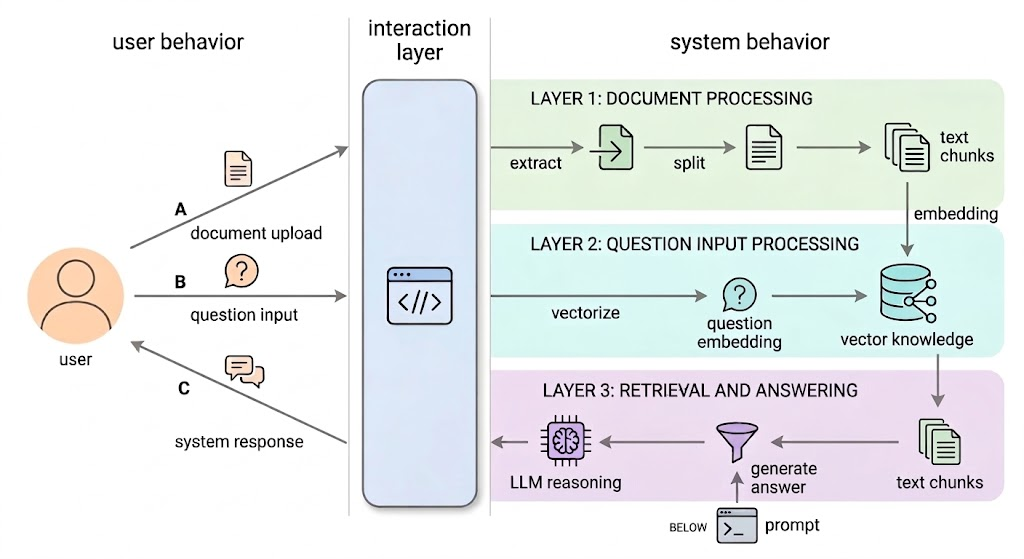
\includegraphics[width=0.8\textwidth]{image/chap02/rag.png}
    \caption{系统概述图}
    \label{fig:hole}
\end{figure}

\section{系统功能需求分析}
\subsection{用户管理}
用户管理模块是本系统的核心安全底座，旨在提供精细化的访问控制与身份验证机制。该模块不仅负责基础的账户生命周期管理，更需通过多维度的权限模型，确保企业私有知识的安全合规使用。
本系统在用户管理模块首先提供基础的用户注册和登录功能，其次通过用户权限区分管理员和普通用户。

另外，针对企业复杂的组织架构，本系统引入组织标签进行多级权限访问控制，通过用户权限和组织标签进行鉴权。
组织标签直接与底层的向量知识库挂钩。当用户发起检索请求时，系统自动提取其对应的组织标签作为检索过滤因子。通过组织标签设置动态的数据访问策略，确保敏感文档在特定的组织范围内流通，从根本上解决企业内部信息越权访问的风险。

用户管理用例如图2.2所示：
\begin{figure}
    \centering
    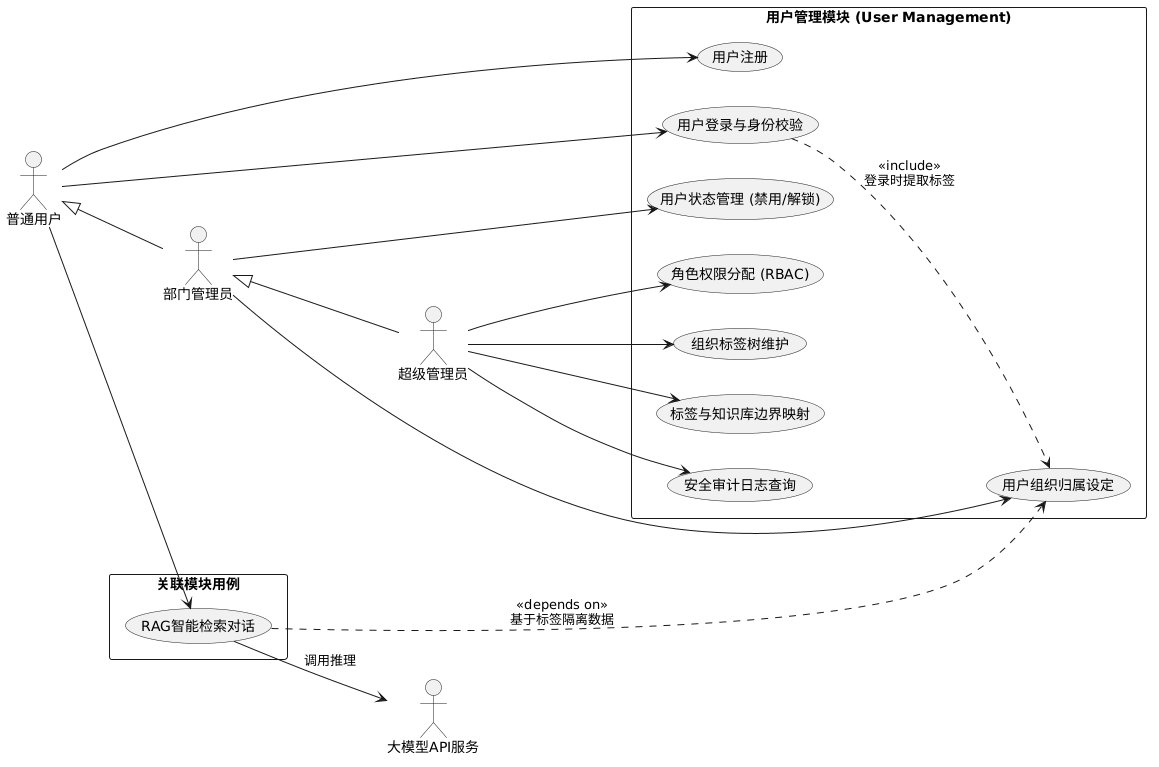
\includegraphics[width=0.7\textwidth]{image/chap02/user.png}
    \caption{用户管理用例图}
    \label{fig:image-embedding-text}
\end{figure}
\subsection{文档处理}
文档处理模块作为本系统知识管理的核心组件，提供非结构化数据向结构化知识资产转化的功能。该模块不仅需提供基础的文档生命周期管理（如增、删、改、查），还需针对企业复杂环境下的大文件传输与数据安全提出针对性解决方案。
首先，系统需构建多租户权限隔离机制。基于前述的组织标签，文档处理模块实现细粒度的访问控制策略，确保用户仅能在其授权范围内进行文档操作，防止跨部门敏感信息的越权泄露。
其次，针对大规模技术文档的传输需求，系统需引入分片上传与断点续传技术。通过在前端进行文件分片预处理，并结合后端的文件指纹（MD5）校验机制，系统能够有效应对网络波动引发的传输中断，提升海量数据入库的稳健性与效率。
最后，文档上传成功后，系统将自动触发自动化知识解析管线。系统将非结构化文本进行语义分段，并利用预训练 Embedding 模型执行向量化映射最终持久化存储至向量数据库中。

文档处理用例如图2.3所示：
\begin{figure}
    \centering
    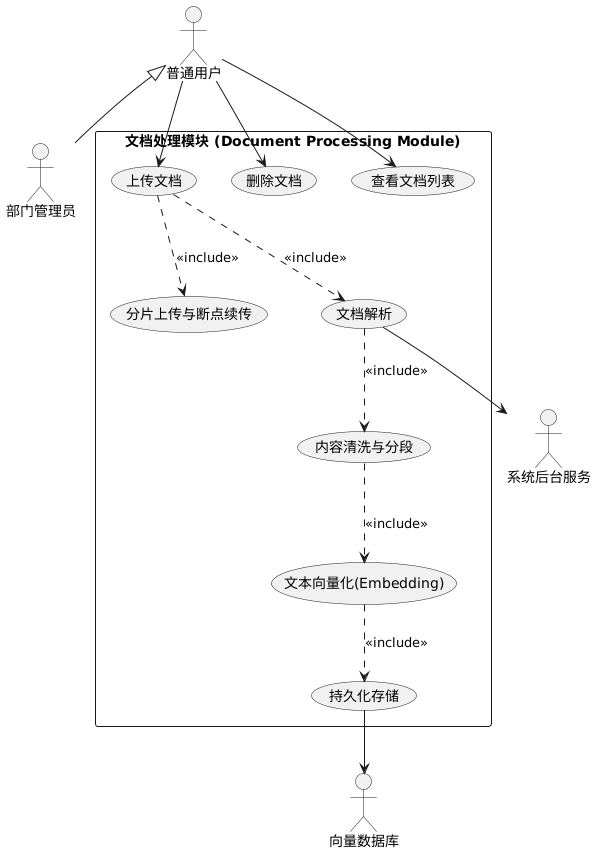
\includegraphics[width=0.6\textwidth]{image/chap02/text.png}
    \caption{文档处理用例图}
    \label{fig:image-embedding-text}
\end{figure}

\subsection{问题处理}
系统通过度量用户提问与知识库文档的语义相似度，自动提取相关知识碎片，并将其作为上下文约束注入生成模型。该流程的首要环节是对用户查询进行高维向量化表征，将其映射至与知识库一致的向量空间，以实现精准的语义对齐。

问题处理用例图如图2.4所示：
\begin{figure}
    \centering
    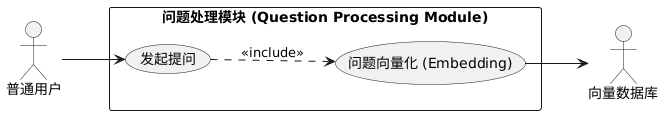
\includegraphics[width=0.6\textwidth]{image/chap02/querry.png}
    \caption{问题处理用例图}
    \label{fig:image-embedding-text}
\end{figure}

\subsection{检索模块}
检索模块作为本系统的核心模块，负责实现用户查询指令与异构知识库之间的语义对齐与高维信息提取。为确保系统在复杂的企业应用场景下具备高可靠性，本研究针对检索精确度与数据访问安全性两项核心指标进行了深度设计。

在检索效能方面，系统弃用了单一的文本匹配模式，构建了基于混合查询式检索（Hybrid Query-Based Retrievers）\cite{Sawarkar_2024}与重排序（Re-ranking）\cite{mortaheb2025rerankingcontextmultimodalretrieval}的协同优化机制。通过融合关键词检索与语义检索的优势，系统能够兼顾长尾词匹配与深度语义理解。随后，利用topK参数对召回的候选文档切片执行二次精排，提升检索结果的查准率。

在安全治理层面，系统引入了基于组织标签的物理与逻辑双重隔离机制。检索引擎在执行向量空间检索前，将强制注入用户所属的组织权限因子作为过滤谓词。该设计确保了检索过程仅在授权的知识域内闭环运行，从根本上杜绝了企业内部敏感信息的垂直越权或水平越权访问。

检索模块的用例图如图2.5所示：
\begin{figure}
    \centering
    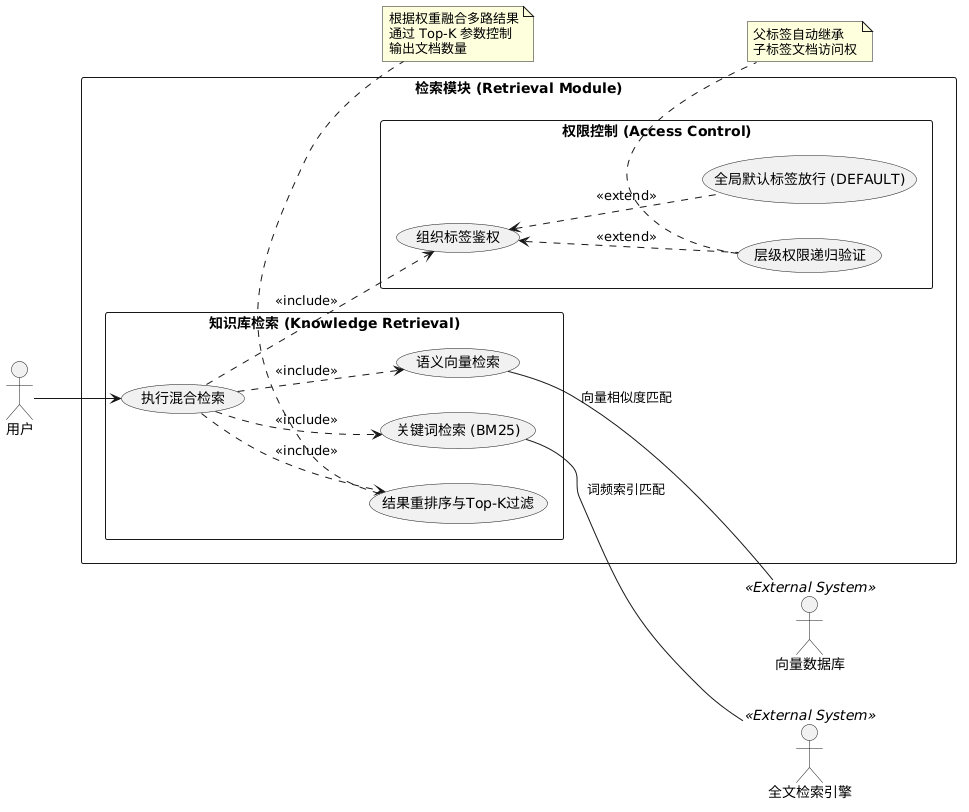
\includegraphics[width=0.8\textwidth]{image/chap02/Retrieval.png}
    \caption{检索模块用例图}
    \label{fig:image-embedding-text}
\end{figure}
\subsection{LLM推理模块}
本系统的生成模块负责将检索阶段获取的候选知识片段与用户原始查询进行深度语义解构与重组。该流程旨在通过高维度的提示词工程\cite{white2023promptpatterncatalogenhance}，构建具备任务导向性的输入序列。

首先，系统建立了一套动态提示词模板库。根据用户意图识别的结果，系统自动化匹配预设的指令模板，并将检索到的异构知识内容嵌入特定上下文槽位。为确保模型输出的严谨性，系统在提示词中预置了系统级约束指令，包括对回答风格、事实溯源要求及负向约束的显式定义。

其次，系统集成了上下文窗口自适应管理机制。针对多轮对话场景，模块通过滑动窗口或语义摘要算法对历史会话进行压缩，确保提示词总量在大型语言模型（LLM）的有效上下文长度范围内。最后，系统构建了模型中台化接口，实现了对 DeepSeek、GPT 等多种异构模型的标准化调用，支持在不同应用场景下进行模型能力的平滑切换与策略对齐。

模型推理模块的用例图如图2.6所示：
\begin{figure}
    \centering
    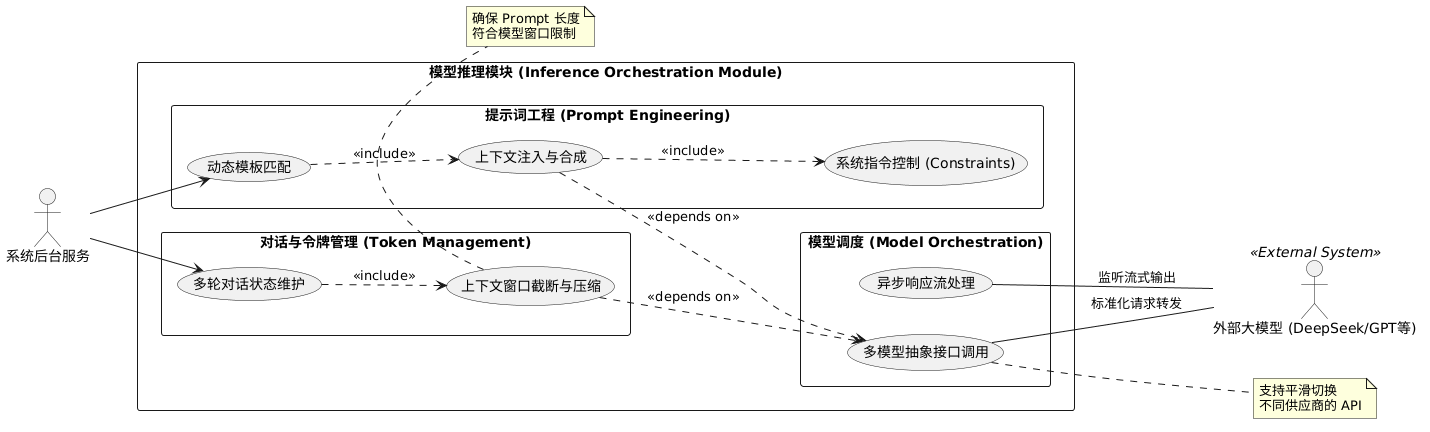
\includegraphics[width=1.1\textwidth]{image/chap02/llm.png}
    \caption{模型推理模块用例图}
    \label{fig:image-embedding-text}
\end{figure}

\subsection{用户交互}
本系统的交互模块遵循 Jakob Nielsen 提出的可用性启发式原则（Usability Heuristics）\cite{nielsen1994inspection}，旨在构建直观、高效且具备容错能力的用户界面。

在会话治理方面，系统实现了完善的会话生命周期管理机制。通过维护全局会话状态栈，系统能够自动捕获并关联历史语境，确保多轮对话中的语义一致性与上下文连贯性。同时，系统为用户提供历史会话的持久化管理功能（如检索、重命名及删除），满足了知识溯源与长周期任务处理的需求。

在交互性能层面，为缓解大语言模型（LLM）推理延迟带来的负面体验，系统采用了流式输出架构。系统能够将生成的 Token 实时推送到前端页面，实现“即时响应”的视觉反馈。这种异步交互范式不仅显著提升了系统的感知性能，也符合尼尔森原则中关于“系统状态可见性”的核心要求\cite{nielsen1994inspection}。

用户交互模块的用例图如图2.7所示：
\begin{figure}
    \centering
    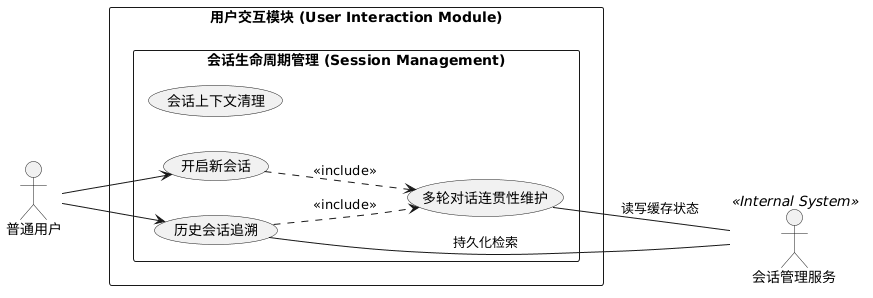
\includegraphics[width=1.0\textwidth]{image/chap02/inter.png}
    \caption{用户交互模块用例图}
    \label{fig:image-embedding-text}
\end{figure}

\section{非功能需求分析}
本研究参照 ISO/IEC 25010 软件质量模型，针对本系统的工程特性，从性能效率、安全性、可靠性及可扩展性四个维度确立了系统的非功能性约束\cite{iso25010_2011}。
\begin{enumerate}
    \item 系统性能主要受控于核心检索推理模块与用户交互模块。针对引入混合检索与重排序带来的额外计算开销，系统设定了严苛的响应时延门限，确保首字响应时间处于感知优良范围内。此外，系统需具备高维向量化处理过程中的 CPU/GPU 负载均衡调度能力，以支撑高并发场景下的吞吐量需求，防止资源争抢导致的系统阻塞。
    \item 鉴于企业知识资产的私密性，安全性构成本系统的核心底座。系统通过组织标签隔离机制防止跨部门数据的越权访问。针对敏感信息，系统对用户输入及模型输出进行双向敏感词过滤，严禁机密内容通过模型推理接口泄露至公网。同时，在静态存储阶段，系统对向量数据库与原始文档库实施强加密传输与存储协议，确保底层数据免受非法读取。
    \item 为保障业务连续性，系统设计了服务容错与平滑降级机制。当大模型 API 或向量存储出现异常时，系统可切换至轻量化本地模型或备用节点。此外，系统需解决文档入库与实时检索间的数据一致性挑战，通过事务流水线管理，确保海量并发写入场景下的数据实效性与检索准确性。
    \item 系统架构设计遵循松耦合与微服务化原则，以适配现有办公生态。随着企业语料库规模的指数级增长，系统支持向量数据库的分布式水平扩展。同时，通过构建模型抽象适配层，系统具备核心组件的“即插即用”能力，支持根据成本与算力需求，在不同供应商的大模型服务间进行无感切换。
\end{enumerate}